% \CQUsection{相关理论基础}

% \CQUsubsection{动脉瘤以及分割基本原理}

% 脑动脉瘤是指脑血管壁局部异常膨出，形成像气球一样的囊状或梭形结构。它最常发生在脑底部的Willis环（大脑主要动脉汇合处）及其分支上。在CTA图像中主要表现为，局部囊状突出：血管壁向外膨出的“气球样”或“浆果样”结构。
% 瘤颈：动脉瘤与载瘤动脉连接的狭窄部位。

% \begin{figure}[htbp]
% 	\centering
% 	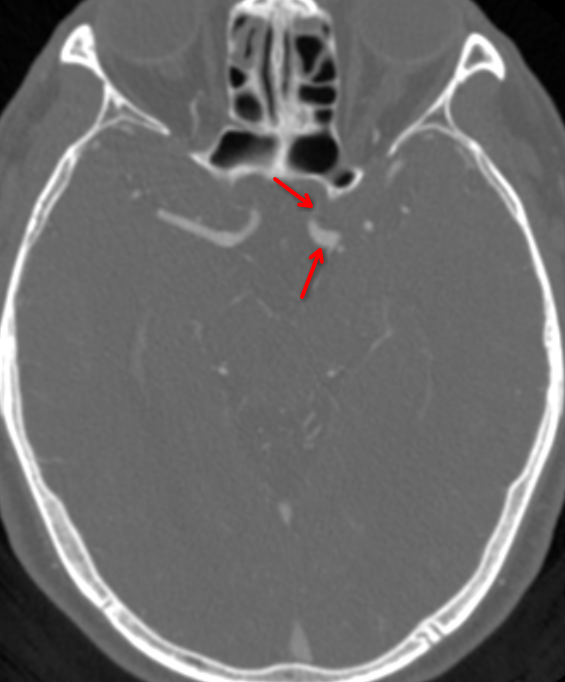
\includegraphics[width=0.4\textwidth]{figure/aneurysm_case.png}
% 	\caption{实际脑动脉瘤样例}
% 	\label{fig:system_architecture}
% \end{figure}

% 从上述图片可见，在上红色箭头所指，可看到模糊血管轮廓，但在下箭头所指，可发现血管突然涨大，是典型的动脉瘤病灶标准。

% \CQUsubsection{医学图像分割基本理论}
% 医学图像分割的目标是在像素或体素层面对目标解剖结构进行精确定位，其本质是一个密集预测问题。与自然图像中的目标检测相比，CTA 体数据具有三维空间连续、前景占比极低、病灶形态差异显著等特点，因此模型不仅需要学习局部边缘与纹理，还要保持跨层空间一致性。对于颅内动脉瘤任务而言，分割结果既可作为病灶可视化依据，也可进一步支持体积、长径、形态不规则度等衍生指标的计算，从而成为后续风险评估的重要输入。

% 在经典监督学习框架下，训练样本由输入图像 $X$ 与金标准标签 $Y$ 构成，模型学习从 $X$ 到 $Y$ 的映射函数 $f_{\theta}(X)$。由于医学图像标注成本高、类别分布不平衡、成像条件复杂，实际训练中往往需要在网络结构、损失函数与采样机制之间协同设计，以保证模型既具有表达能力，又能稳定收敛。

% \CQUsubsection{卷积神经网络与 U-Net 结构}
% 卷积神经网络（Convolutional Neural Network, CNN）通过局部感受野、权值共享和层级特征提取机制，在图像分析任务中取得了广泛应用。对于分割问题，FCN（Fully Convolutional Network）首先将分类网络推广到像素级预测，使网络能够直接生成密集输出图\cite{long2015}；而 U-Net 在此基础上引入对称的编码器—解码器结构及跳跃连接，使浅层细节信息与深层语义信息得以融合，显著提升了医学图像分割精度\cite{unet}。

% 三维医学图像具有明显的层间连续性，因此三维卷积网络能够更自然地利用上下文信息。3D U-Net 将二维卷积替换为三维卷积与三维上采样，可同时建模切片内与切片间的空间关系\cite{unet3d}。然而，三维卷积也会带来更高的显存与计算开销，因此在实际工程实现中通常需要结合补丁采样、流式加载和混合精度等策略来控制资源消耗。

% \CQUsubsection{注意力机制与 Attention U-Net}
% 注意力机制的核心思想是让模型在大量候选特征中自适应地突出与当前任务更相关的部分。对于颅内动脉瘤分割任务，病灶体积小、背景血管复杂，若直接拼接所有跳跃连接特征，容易将大量与病灶无关的响应传递至解码器，增加误检风险。Attention U-Net 在跳跃连接处加入门控模块，对编码器特征进行筛选，使解码器更关注目标区域\cite{attention_unet}。

% 从形式上看，注意力门控通过当前解码特征与同尺度编码特征的联合映射生成一张权重图，再对编码特征进行加权。该机制可以理解为一种空间相关性筛选：当某位置更可能属于动脉瘤或其邻近血管区域时，权重会相对提高；当某位置更可能是背景时，权重会被抑制。这样既有助于减少无关背景干扰，又保留了 U-Net 对局部边界细节的表达优势。

% \CQUsubsection{类别不平衡与损失函数基础}
% 在颅内动脉瘤任务中，目标体素通常只占整例 CTA 体积中的极小比例，属于典型的类别极不平衡问题。若仅使用标准交叉熵损失，模型很容易学到“全部预测为背景”这一平凡解，从而在总体准确率上表现较高，却难以真正检出病灶。因此，需要引入更关注前景重叠程度的区域型损失。

% Dice 系数是衡量预测区域与真实区域重叠程度的常用指标，其对应的 Dice 损失能够直接优化前景区域的一致性。对于预测概率 $p_i$ 与标签 $g_i$，Dice 损失可写为：
% \begin{equation}
% \mathcal{L}_{Dice}=1-\frac{2\sum_i p_i g_i+\epsilon}{\sum_i p_i+\sum_i g_i+\epsilon},
% \end{equation}
% 其中 $\epsilon$ 为平滑项。交叉熵损失则从逐体素分类角度约束模型输出，强调概率预测的数值稳定性。将二者组合能够兼顾局部分类准确性与整体区域重叠度，这也是本文分割模块损失设计的理论基础。

% 对于风险预测任务，破裂与未破裂样本往往同样存在比例失衡，因此二分类训练中需要通过正类加权、阈值搜索等方式提高模型对少数类的敏感性。相比固定阈值 0.5，基于验证集的阈值搜索能够在精确率与召回率之间取得更符合任务目标的平衡。

% \CQUsubsection{表格学习与特征表示理论}
% 除影像体数据外，临床信息、人口统计学特征与既往病史通常以结构化表格形式存在。传统表格学习方法如逻辑回归、支持向量机和随机森林在变量规模有限时具有一定优势，但在数值特征与类别特征混合、非线性交互显著的场景下，模型表达能力可能受到限制。

% 近年来，深度表格学习开始借鉴自然语言处理中的 token 化思想：将每个数值字段、类别字段都映射为统一维度的隐向量，再利用注意力机制建模字段之间的交互关系。其优点在于：一方面避免了人工构造高阶交叉项，另一方面能够统一处理连续变量与离散变量，为多模态融合提供了更灵活的表示空间。本文风险模型即基于这一思想，将数值 token 与类别 token 送入交叉注意力模块，以学习临床变量之间的潜在关联。

% \CQUsubsection{评价指标基础}
% 分割与分类任务的评价重点不同。分割侧常用 Dice 系数、敏感度、特异度、Hausdorff 距离等指标，其中 Dice 强调重叠区域的一致性，适合评价前景区域的整体拟合程度。分类与风险预测侧则常用准确率、精确率、召回率、F1 值与 AUC。AUC 反映模型对正负样本排序能力的整体水平，而 F1 值综合考虑精确率与召回率，适合在类别不平衡场景下衡量模型的综合表现。

% 需要指出的是，对于极度稀疏的医学分割任务，单独依赖总体准确率往往会产生误导，因为背景体素数量远大于前景体素数量。正因如此，本文在实验分析中同时报告 Dice、体素级 F1、多阈值统计与基于直方图近似的 voxel AUC，以尽可能全面地反映模型性能。

% \CQUsubsection{本章小结}
% 本章围绕本文后续方法设计所依赖的理论基础进行了概述，主要包括三维医学图像分割的基本问题、CNN 与 U-Net 结构、注意力门控机制、类别不平衡下的损失函数设计、表格特征表示与交叉注意力思想，以及分割和风险预测常用评价指标。上述理论共同构成了本文系统实现与实验分析的出发点，为下一章的模型设计与工程实现提供了方法依据。




\CQUsection{相关理论基础}

\CQUsubsection{脑动脉瘤及分割基本原理}

脑动脉瘤是指脑血管壁局部异常膨出所形成的囊状或梭形结构，最常发生于脑底部的Willis环及其主要分支。在CTA图像中，脑动脉瘤的主要表现为血管壁的局部囊状突出，呈现为“气球样”或“浆果样”的异常膨出结构。

其中，瘤颈（neck）是指动脉瘤与载瘤动脉之间的连接部位，其宽度和形态对临床诊断具有重要意义。

\begin{figure}[htbp]
	\centering
	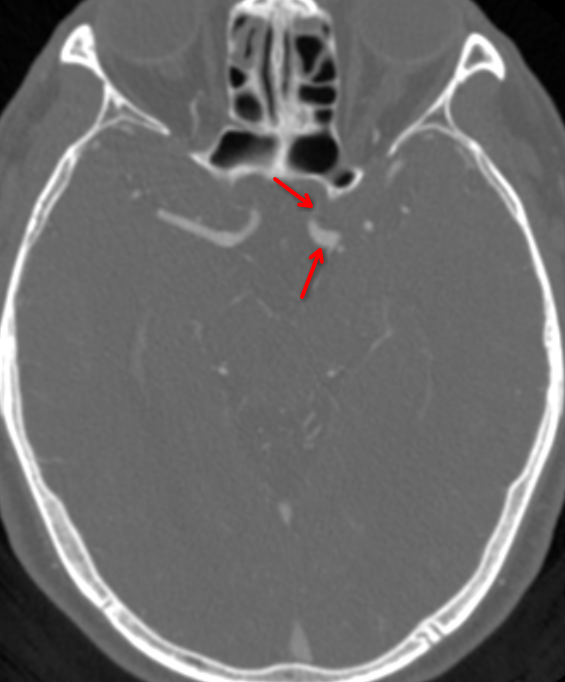
\includegraphics[width=0.45\textwidth]{figure/aneurysm_case.png}
	\caption{实际脑动脉瘤CTA影像示例}
	\label{fig:aneurysm_case}
\end{figure}

如图所示，红色箭头指示区域中，上方血管轮廓相对正常，而下方箭头所指位置可见血管突然异常膨大，呈现典型的脑动脉瘤病灶特征。

\CQUsubsection{医学图像分割基本理论}

医学图像分割旨在像素或体素层面实现对目标解剖结构的精确定位，本质上属于密集预测（dense prediction）任务。与自然图像分割不同，CTA体数据具有三维空间连续性、前景占比极低以及病灶形态变异大等特点。因此，模型不仅需要捕捉局部边缘与纹理信息，还必须维持跨层面的空间一致性。该研究范式已在医学影像深度学习综述中得到明确论证\cite{litjens2017survey,shen2017deep,maier2019learning}。

从数学形式上看，三维医学图像分割可表示为对每个体素位置 $u\in\Omega$ 的类别估计问题，其中 $\Omega$ 表示体数据的空间定义域。模型需要学习条件概率 $p(y_u=1\mid X)$，并据此生成概率图 $P=\{p_u\}_{u\in\Omega}$。当给定阈值 $\tau$ 时，二值分割结果可由 $\hat{y}_u=\mathbb{I}(p_u\geq\tau)$ 得到。在此过程中，分割模型既需要输出具有空间连续性的概率分布，又要在局部边界处保持足够的敏感性，以便后续的风险预测模型准确捕捉病灶形态细节。

对于颅内动脉瘤分割任务而言，精确的分割结果既能为临床提供直观的可视化依据，也可进一步计算瘤体体积、最大径、形态不规则度等量化指标，成为后续破裂风险评估的重要基础。

在经典监督学习框架下，训练样本由输入图像 $X$ 和金标准标签 $Y$ 构成，模型的目标是学习从 $X$ 到 $Y$ 的映射函数 $f_{\theta}(X)$。由于医学图像标注成本高、类别分布极度不平衡以及成像条件复杂，实际训练中需在网络结构、损失函数和采样策略上进行权衡，以平衡模型的表达能力和训练稳定性。

\CQUsubsection{卷积神经网络与 U-Net 结构}

卷积神经网络（CNN）通过局部感受野获取到对层次化特征的高效利用，因此在医学图像分析中得到广泛应用。对于分割任务，Fully Convolutional Network（FCN）首次将分类网络扩展至像素级预测，实现端到端的密集输出\cite{long2015}。U-Net则在此基础上引入对称的编码器—解码器结构和跳跃连接（skip connection），有效融合浅层细节信息与深层语义信息，显著提升了医学图像分割性能\cite{unet}。

鉴于三维医学图像在层间具有较强的连续性，3D U-Net将二维卷积替换为三维卷积和三维上采样，从而能同时捕捉切片内部和切片之间的空间上下文信息\cite{unet3d,cciccek20163d}。在后续出现的 V-Net、UNet++ 与 nnU-Net 在体素级残差建模、跳跃连接设计以及自动化配置等方面做了改进，进一步提升了医学图像分割的性能\cite{milletari2016,zhou2018unetpp,nnunet}。不过，三维卷积同时也带来了更高的计算和显存开销，因此实际应用中常采用补丁训练（patch-based training）、流式加载及混合精度训练方法缓解此问题。

\CQUsubsection{注意力机制与 Attention U-Net}

注意力机制的核心在于使模型能够自适应地聚焦于与当前任务最相关的特征区域。对于体积小、背景血管复杂的颅内动脉瘤分割任务，若直接拼接所有跳跃连接特征，易将大量无关背景响应传递至解码器，增加误分割风险。Attention U-Net在跳跃连接处引入注意力门控（Attention Gate）模块，对编码器特征进行筛选，使解码器更关注目标相关区域\cite{attention_unet}。

从实现机制来看，注意力门控将解码器特征与同尺度编码器特征进行融合映射，生成一张空间权重图，再使用生成的权重图对编码器特征进行加权。本质上它完成了空间特征筛选的作用：当某位置更可能属于动脉瘤或邻近血管时，权重被提升；反之则被抑制。通过这种方式，模型在减少背景干扰的同时，较好地保留了U-Net对局部边界细节的敏感性。

\CQUsubsection{类别不平衡与损失函数设计}

颅内动脉瘤在CTA体数据中通常仅占极小比例（往往不足0.1\%），且其分布不均匀。若仅采用标准交叉熵损失，模型容易陷入“全部预测为背景”的平凡解，导致整体准确率虚高而病灶检出能力不足。因此，需要引入侧重前景区域重叠的损失函数。

在损失函数设计上，常见做法是在二元交叉熵（BCE）的基础上引入区域重叠型损失或难分割病例挖掘型损失\cite{sudre2017generaliseddice,salehi2017tversky,lin2017focal}。其中，Tversky 损失是 Dice 损失在假阳性与假阴性惩罚权重上的推广，在训练过程中，Tversky 损失往往比 Dice 损失更敏感，更关注于分割结果中的边界，其定义如下：

\begin{equation}
\mathcal{L}_{\text{Tversky}} = 1 - \frac{TP + \epsilon}{TP + \alpha FP + \beta FN + \epsilon},
\end{equation}

其中 $TP$、$FP$、$FN$ 分别表示软预测意义下的真阳性、假阳性和假阴性，$\alpha$ 与 $\beta$ 控制两类错误的相对权重，$\epsilon$ 为平滑系数。当任务更关注降低漏检时，可适当提高假阴性项的惩罚权重；当任务更关注减少误检时，则可提高假阳性项的惩罚权重。Focal 损失则通过降低易分类样本的损失贡献，使优化过程更加关注难分类体素。上述损失函数从不同角度缓解前景稀疏问题，为后续分割模型的训练目标设计提供了理论依据。

对于后续的动脉瘤破裂风险预测任务，由于正负样本同样存在不平衡，通常需采用正类加权或基于验证集的阈值优化策略，以提升模型对少数类（破裂组）的敏感性。

\CQUsubsection{表格数据学习与特征表示理论}

除了影像数据外，临床信息、人口统计学特征和既往病史等通常以结构化表格的形式存储。传统机器学习方法（如逻辑回归、随机森林）在特征维度较低时表现不错，但面对高维混合特征（数值型+类别型）以及复杂的非线性交互时，表达能力会明显受限。

近年来，深度表格学习借鉴NLP中的Token化思想，将每个特征字段映射为统一维度的隐向量，再通过注意力机制捕捉字段间的交互关系。其中，TabTransformer 利用上下文化嵌入增强了类别变量表达能力，FT-Transformer 则进一步验证了对数值字段进行 token 化并使用 Transformer 编码的有效性\cite{tabtransformer2020,fttransformer2021}。这类方法无需人工构造高阶交叉特征，且能统一处理连续与离散变量，为多模态融合提供了灵活高效的方案。

本文的风险预测模块即基于这一思路构建；同时，我也保留了随机森林和梯度提升树等传统集成学习方法作为小样本表格数据上的重要对比基线\cite{breiman2001rf,chen2016xgboost,hastie2009elements}。

\CQUsubsection{临床风险评分与深度模型的互补关系}

未破裂颅内动脉瘤的管理并非单纯的图像分割问题。PHASES 评分综合人群来源、高血压、年龄、动脉瘤大小、既往蛛网膜下腔出血史和部位等因素，用于估计未来破裂风险\cite{greving2014}；ELAPSS 评分则将年龄、部位、大小、形态和既往蛛网膜下腔出血等因素纳入未破裂动脉瘤增长风险预测\cite{backes2017}。此外，大规模自然病程队列研究也提示，不同部位、不同直径和形态不规则程度的动脉瘤具有不同的破裂倾向\cite{morita2012,thompson2015}。

上述评分体系具有解释性强、使用门槛低的优点，但其变量项相对固定，难以充分吸收三维分割衍生出的体积、表面不规则度、瘤颈宽度、影像组学纹理等高维信息。深度学习模型则可在数据充分且划分严格的前提下学习非线性交互。因此，将注意力表示学习与传统机器学习方法进行比较或融合，有助于同时考察非线性表征能力与小样本稳健性，并为风险预测提供更全面的方法学参照。

\CQUsubsection{评价指标基础}

分割任务常用Dice系数、敏感度（Sensitivity）、特异度（Specificity）、Hausdorff距离等指标，其中Dice系数重点衡量预测区域与真实区域的重叠程度。分类与风险预测任务则常用准确率、精确率、召回率、F1值以及AUC-ROC等指标。AUC反映模型整体排序能力，F1值则在不平衡场景下更能综合体现精确率与召回率的平衡。鉴于医学管理系统中，对病灶的漏诊远远严重于误诊，因此，本文选择使用召回率来进行模型的首要评判标准，兼用AUC进行模型性能评估。

针对极度稀疏的医学分割任务，单纯依赖总体准确率易产生误导。因此，在实验代码中同时报告Dice系数、体素级F1、多阈值统计结果及基于直方图近似的voxel-wise AUC，以实现对模型性能的全面评估；同时在这种不平衡二分类场景中PR曲线与校准分析同样具有重要参考价值\cite{saito2015pr,guo2017calibration,niculescumizil2005calibration,chicco2020f1}。

\CQUsubsection{本章小结}

本章系统概述了本文研究所需的核心理论基础，包括脑动脉瘤的影像学表现、三维医学图像分割基本问题、U-Net及其注意力变体、类别不平衡下的损失函数设计、表格数据深度表征方法，以及相关评价指标体系。这些理论为后续章节的模型设计、优化策略与实验分析提供了坚实的理论支撑。

